\section{Detrending absorption spectrum and identification of lines}
The given task should only be done for one temperature. The chosen temperature is $60^\circ\,$C in our measurement because here 
the lines are clear in comparison with the other temperatures. Also, the peaks at the temperature $60^\circ\,$C are the best defined ones. 
$60^\circ\,$C was the desired temperature, however we only could get a temperature of $(56.0\pm 0.2)^\circ\,$C.\\
\subsection{Cleaning the data}
First of all, the mess data should be considered. Therefore, have a closer look at the following plot:\\
\begin{center}
    \begin{figure}[h]
        \centering
        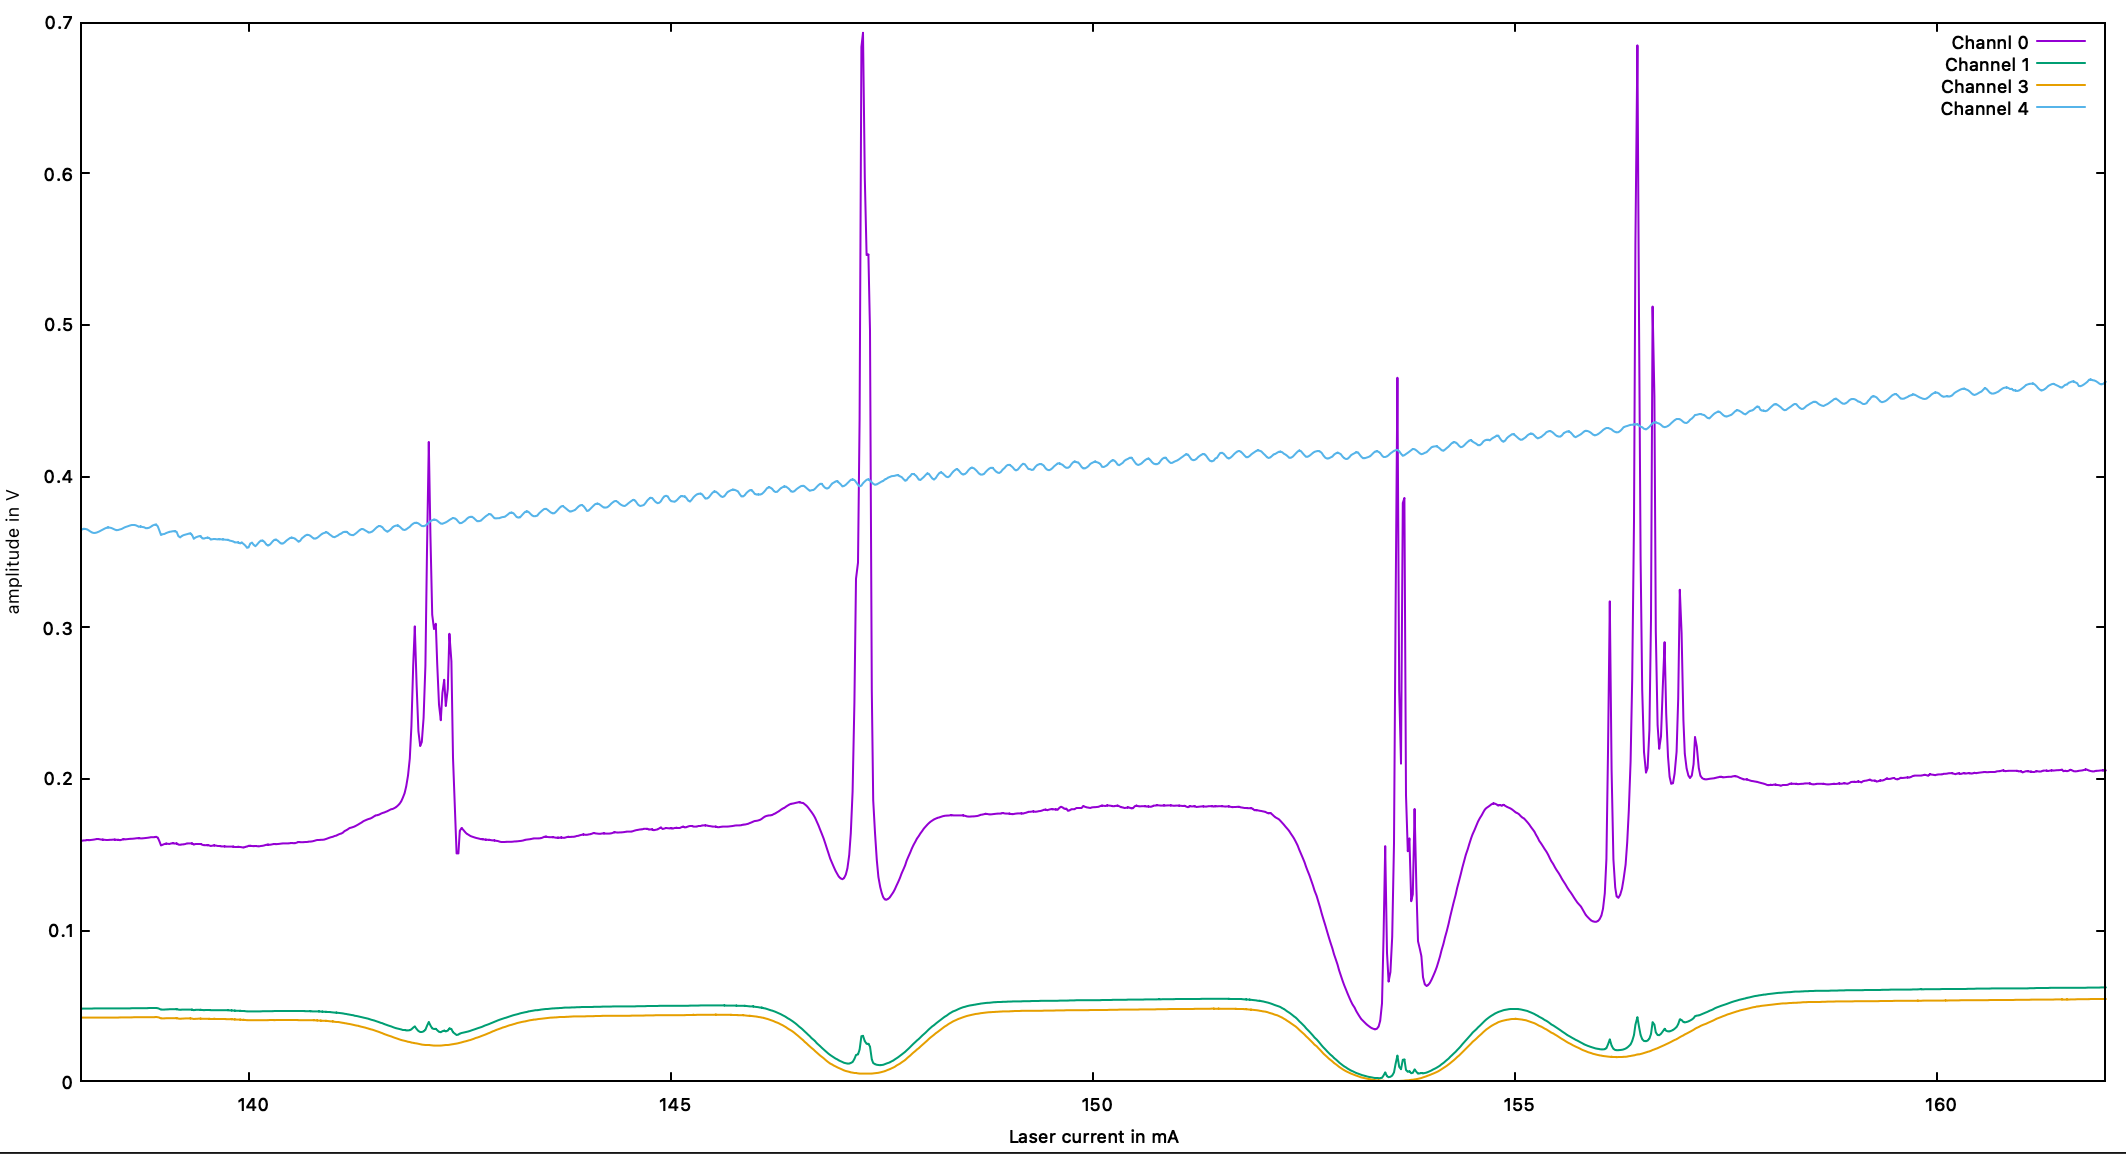
\includegraphics[scale=0.4]{Bilder/Auswertung_Anna/L_normal.png}
        \caption{unadjusted mess data}
        \label{fig:unadjusted}
    \end{figure}
\end{center}
In this plot channel 0 is the Difference, channel 1 is the absorption spectrum, channel 3 is the reference measurement and
channel 4 is the Fabry Perot Interferometer.\\

As can be seen from the plot, the measured values appear to be subject to a slight slope.
This increasing trend seems to distort them. 
So, it's obvious that the measured data need to be adjusted and freed from this trend.
In order to be able to implement this, one must first fit a straight line at the increasing trend.
Afterwards this straight line will be subtracted from the mess data and we receive the trend-free and adjusted data. 
\newpage
Unfortunately, the slope of the increasing trend is only in the channel 0, channel 1 and channel 3 similar. 
Accordingly, you have to calculate a second fit-line and apply it only to channel 4.\\
\textbf{First fitting line:}\\
For the first fitting line (for the channel 1, channel 2 and channel 3) we use only one channel 
to do the fitting line. We can apply this fitting-line to the other mess data as well, since as already mentioned above, 
the slope of the three channels is similar.\\
After the fit has just been determined, the program GNUplot is used for this purpose, 
we subtract the line from the mess data. \\
The following plot is intended to illustrate as an example how the just described progress proceed:\\
\begin{center}
    \begin{figure}[h]
        \centering
        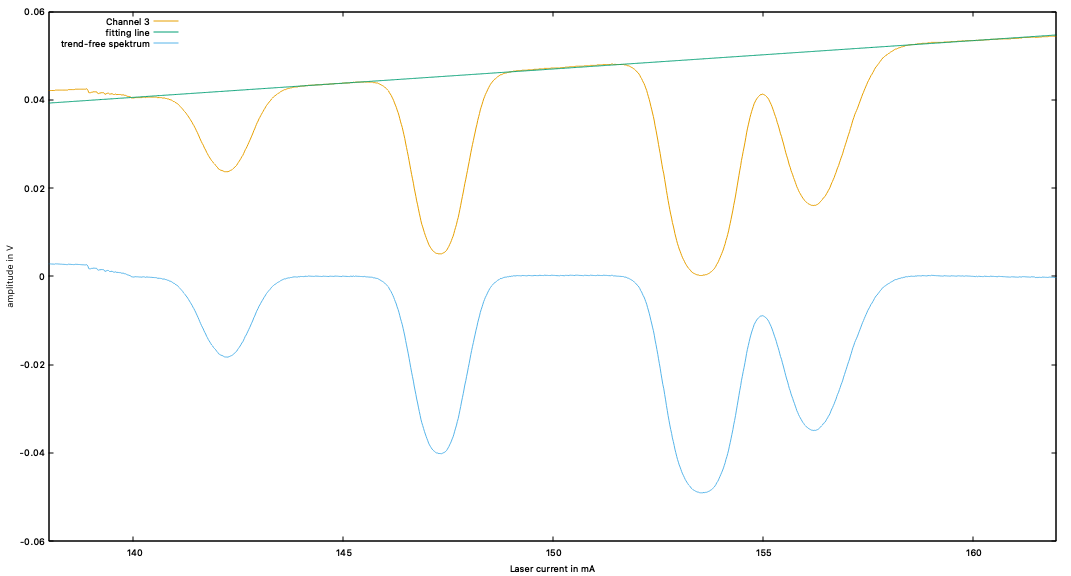
\includegraphics[scale=0.3]{Bilder/Auswertung_Anna/clean_ch3.png}
        \caption{unadjusted data (orange), fitting line (green) and trend-free data (blue).}
        \label{fig:ch3_clean}
    \end{figure}
\end{center}
This is done for the rest of the data as well, but not shown explicitly again.\\
\textbf{Second fitting line:}\\
For the fitting line for channel 4 we use as well GNUplot.
After we found the correct fitting line, we subtract this line as well from the original 
mess data to get the adjusted mess data.
\begin{center}
    \begin{figure}[h]
        \centering
        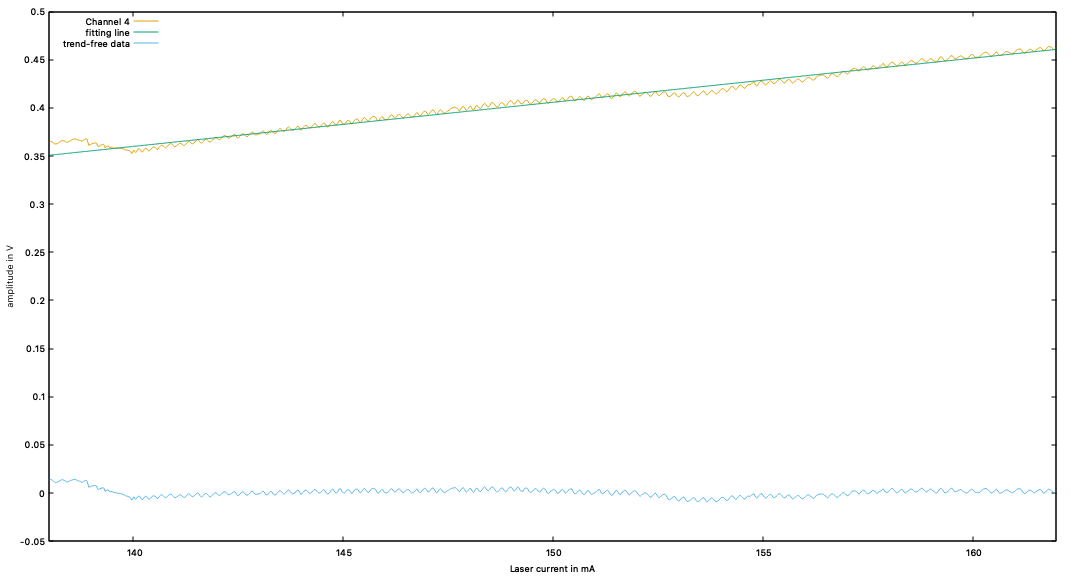
\includegraphics[scale=0.3]{Bilder/Auswertung_Anna/clean_ch4.png}
        \caption{unadjusted mess data (orange), fitting line (green) and adjusted mess data (blue) of channel 4 }
        \label{fig:ch4_clear}
    \end{figure}
\end{center}
The following plot shows, why it was necessary to do a second fitting line:\\
\begin{center}
    \begin{figure}[h]
        \centering
        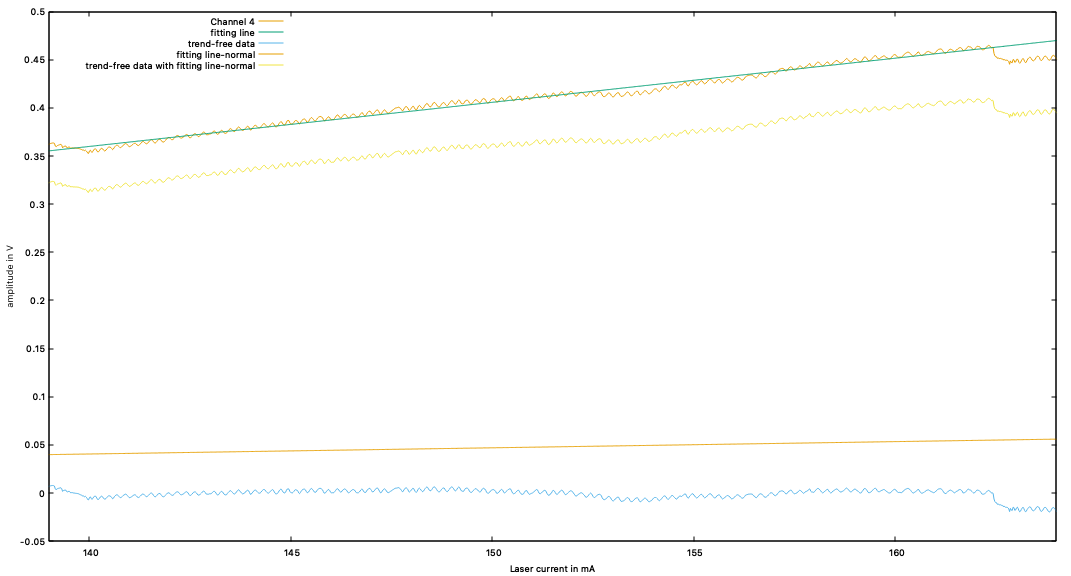
\includegraphics[scale=0.3]{Bilder/Auswertung_Anna/all_ch4.png}
        \caption{first fitting line (orange) and second fitting line (green) of channel 4 in comparison}
        \label{fig:ch4_all}
    \end{figure}
\end{center}
As you can see from this plot, it was necessary to calculate a new fitting line.
The fitting line (orange) for the channels 0, 1 and 3 has a too low fitting line gradient to really clean up
the FPI data. So a second line (green) was calculated and we receive 
the adjusted mess data (blue) of channel 4. \\
At the end the whole adjusted mess data for all channels look like:\\
\begin{center}
    \begin{figure}[h]
        \centering
        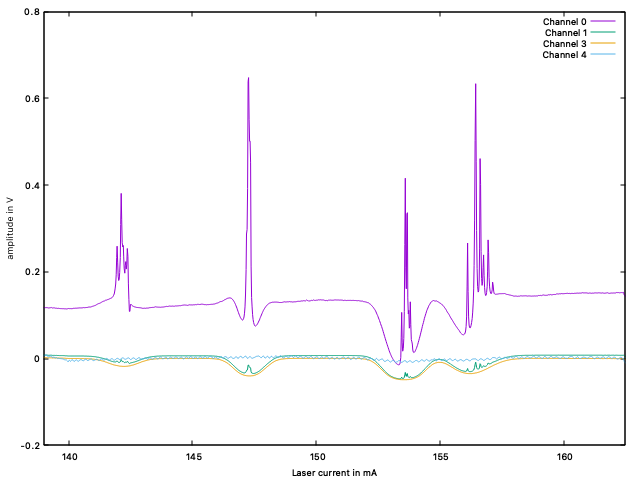
\includegraphics[scale=0.5]{Bilder/Auswertung_Anna/clean_all.png}
        \caption{adjusted mess data for all channels}
        \label{fig:all}
    \end{figure}
\end{center}
\newpage
\subsection{identification of the lines and transmission}
In the next sub-task, the lines in the absorption spectrum should be named.
First of all, we limit the scan range again, instead of using the full scan range we will only 
be using the area from $140\,$mA to $160\,$mA. We determined that area because there is 
no visible mode jump in between. \\
To define the peaks in the spectrum we fit a Gauss curve over the four lines, for this
we are using Python.
\begin{center}
    \begin{figure}[h]
        \centering
        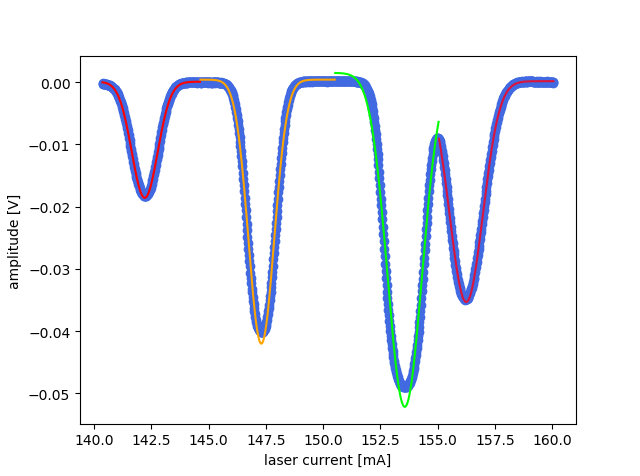
\includegraphics[width=0.8\textwidth]{Verbesserung/plot_all_gauss_ma.png}
        \caption{Gaussian fitting curve for the different peaks}
        \label{fig:gauss}
    \end{figure}
\end{center}
Using a python script you get the exact position of the dips (I in mA) in the spectrum. 
With the help of the Laser current - wavelength relation 
it is possible to convert the current into wavelength. 
\newpage
\begin{center}
    \begin{figure}[h]
        \centering
        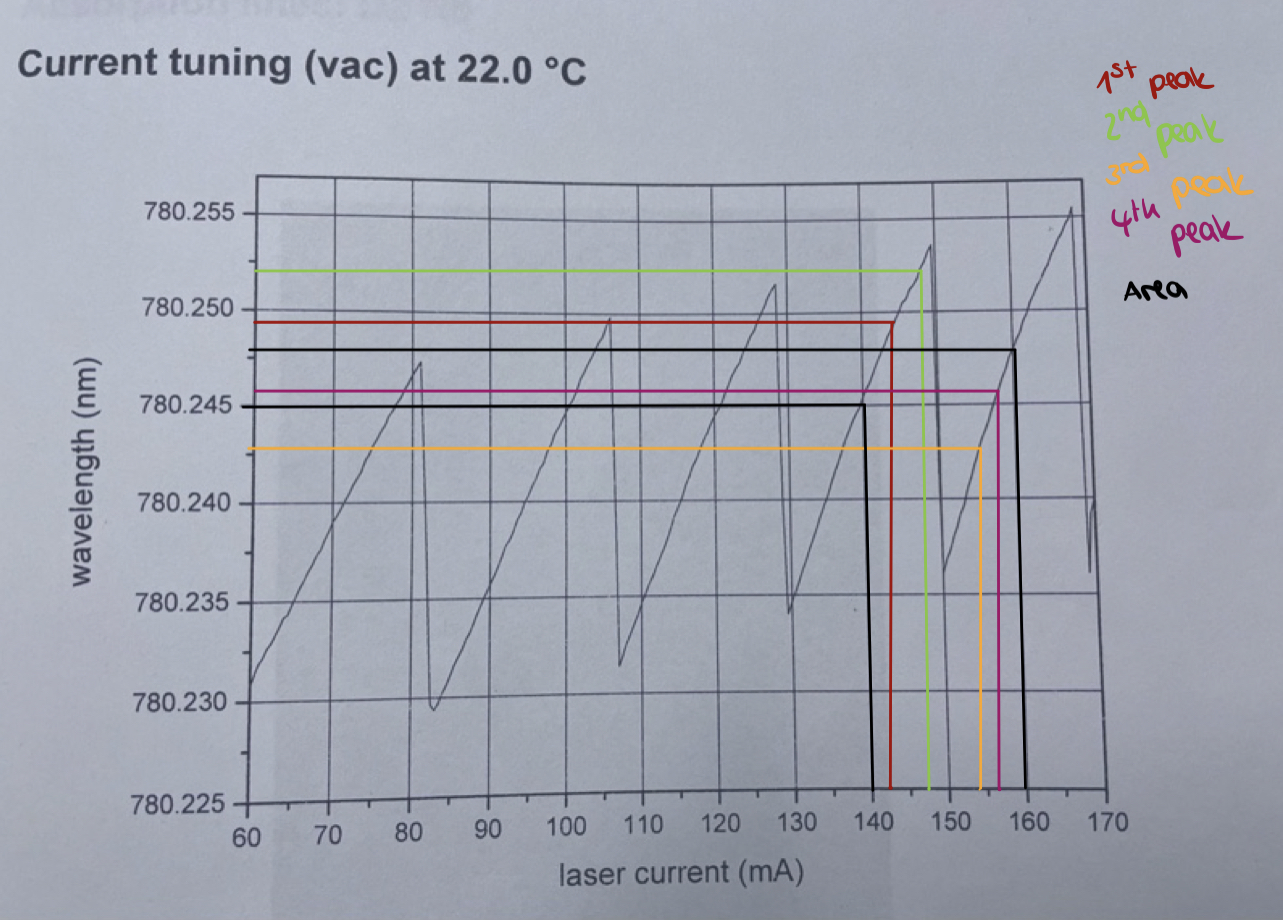
\includegraphics[scale=0.3]{Bilder/Auswertung_Anna/laser-wavelength.jpg}
        \caption{conversion between laser current and wavelength of the laser}
        \label{fig:currentwave}
    \end{figure}
\end{center}
As you can see from the figure \ref{fig:currentwave} it's challenging to find out the exact wavelengths from the
photographed current-wavelength relation. The extracted values are inaccurate and have a big error. 
Therefore, a read-off error of $s_{\lambda} = 0.0005 \text{nm}$ is set.
Nevertheless, we determined as best as possible the wavelength and afterwards we calculated it into the frequency 
with the following equation:
\begin{equation}
    \nu = \frac{c}{\lambda} = \frac{299792458\,\frac{\text{m}}{\text{s}}}{\lambda}
\end{equation}
Here stands c for the speed of Light.\\
The error propagation for the frequency:
\begin{equation}
    s_{\nu} = \frac{c}{\lambda^2} \cdot s_{\lambda} = 0.0000025 \cdot 10^{14}\,Hz
\end{equation}
The results are shown in the following table:\\
\begin{table}[h]
\centering
    \begin{tabular}{c||c|c|c}
        Peak & $I$ in mA & $\lambda$ in nm & $\nu\,\text{in} 10^{14}$ Hz\\
        \hline
      1 & 142.2 & 780.2490 $\pm  0.0005$ & 3.8422665 $\pm  0.0000025$\\
      2 & 147.3 & 780.2522 $\pm  0.0005$ & 3.8422507 $\pm  0.0000025$\\
      3 & 153.6 & 780.2426 $\pm  0.0005$ & 3.8422979 $\pm  0.0000025$\\
      4 & 156.2 & 780.2462 $\pm  0.0005$ & 3.8422803 $\pm  0.0000025$\\
    \end{tabular}%
    \caption{Laser current, wavelength and frequency of the four peaks}
    \label{tab:laser current}%
\end{table}\\
Now that we have determined the wavelengths and frequencies of our lines, 
we have to compare them with appropriate literature values \citep[see][]{AnhangA, AnhangB}.
\newpage
Since in the table \ref{tab:laser current} only a wavelength of approx. $780\,\text{nm}$ appears, 
which is not surprising considering which laser we used during the experiment, 
the literature values are only those of a D2-line.\\
\begin{table}[h]
    \centering
    \begin{tabular}{c|c|c}
      Isotopes & F & $\nu_{lit}\,\text{in} 10^{14}$ Hz\\
      \hline
      \ce{^{87}Rb}& 2 & 3.842279 \\
      \ce{^{85}Rb}& 3 & 3.842291 \\
      \ce{^{85}Rb}& 2 & 3.842321 \\
      \ce{^{87}Rb}& 1 & 3.842348 \\
    \end{tabular} \caption{Literature value for the frequency of transitions}
    \label{tab:litvalue}%
\end{table}\\
The next step is to compare the literature values with ours and then we should
be able to determine the lines.\\
But unfortunately, even if we consider our values and their error bars 
with the literature values they don't match. \\
One possible reason for this might be that the given laser-current characterstic 
is not so accurate for current configuration.
We used an area between two mode jumps, so it's naturally to think that there is an increasing of
the wavelength along to first to fourth peak.
So, as we just discussed the wavelength should be increasing, so the frequency should be decreasing. 
However, if you expand the error range and keep the recently discussed arguments in mind, we can identify the lines: \\
\begin{table}[h]
    \centering
    \begin{tabular}{c|c|c|c}
    Peak & Isotopes & F & $\nu\,\text{in} 10^{14}$ Hz\\
      \hline
      1 & \ce{^{87}Rb}& 1& 3.8422979 \\
      2 & \ce{^{85}Rb}& 2 & 3.8422803\\
      3 & \ce{^{85}Rb}& 3 & 3.8422665 \\
      4 & \ce{^{87}Rb}& 2 & 3.8422507 \\
      \end{tabular}%
    \caption{identification of the Lines}
    \label{tab:lines}%
\end{table}%
\newpage
